\documentclass[aspectratio=169]{beamer}
\usepackage[utf8]{inputenc}
\usepackage[T1]{fontenc}
\usepackage{amsmath,amssymb}
\usepackage{graphicx}
\usepackage{booktabs}
\usepackage{xcolor}
\usepackage{hyperref}
\usepackage{tabularx}
\usepackage{tikz}
\usetikzlibrary{shapes.geometric, arrows, positioning}

\usetheme{Madrid}
\usecolortheme{default}

\definecolor{kaggleteal}{RGB}{32,191,196}
\setbeamercolor{structure}{fg=kaggleteal}

\title{Hull Tactical Market Prediction}
\subtitle{Tactical Asset Allocation with Machine Learning}
\author{Jacopo Dardini}
\date{\today}

\begin{document}

% ===== Slide 1: Title =====
\begin{frame}
\titlepage
\end{frame}

% ===== Slide 2: Outline =====
\begin{frame}{Outline}
\tableofcontents
\end{frame}

% ==============================================================================
% SECTION 1: Introduction & Overview
% ==============================================================================
\section{Introduction \& Overview}

% ===== Slide 3: Competition Overview =====
\begin{frame}{The Kaggle Challenge}
\begin{itemize}
    \item \textbf{Goal}: Predict daily S\&P 500 excess returns and convert to weights in $[0, 2]$
    \item \textbf{Metric}: Adjusted Sharpe ratio (penalizes risk and underperformance)
    \item \textbf{Data}: Anonymized macroeconomic, sentiment, and pricing features ($\sim$9k days)
    \item \textbf{Constraint}: Weights must be between 0 and 2; predictions evaluated daily
\end{itemize}
\vspace{0.2cm}
\begin{block}{Why this matters}
    Tactical asset allocation adjusts market exposure based on predictive signals. The adjusted Sharpe metric is useful here because it penalizes both excess risk and falling behind the market.
\end{block}
\end{frame}

% ===== Slide 4: The Adjusted Sharpe Metric =====
\begin{frame}{Adjusted Sharpe Ratio}
\begin{align*}
    \text{adjusted\_sharpe} &= \frac{\text{Sharpe}}{\text{vol\_penalty} \times \text{return\_penalty}} \\[0.1cm]
    \text{vol\_penalty} &= 1 + \max\left(0,\; \frac{\sigma_{\text{strat}}}{\sigma_{\text{mkt}}} - 1.2\right) \\[0.05cm]
    \text{return\_penalty} &= 1 + \frac{\text{gap}^2}{100} \\[0.05cm]
    \text{gap} &= \max\bigl(0,\; (\mu_{\text{mkt}} - \mu_{\text{strat}}) \times 100 \times 252\bigr)
\end{align*}
\vspace{0.05cm}
\begin{block}{Key insight}
    The \textbf{quadratic} return penalty makes sustained underperformance expensive (falling 5\% behind multiplies the denominator by $\sim$1.25). The strategy \textbf{defaults to index exposure} ($w = 1.0$) unless the signal is strong enough.
\end{block}
\end{frame}

% ===== Slide 5: Data Overview =====
\begin{frame}{Data Description}
\begin{itemize}
    \item \textbf{Train set}: 8\,990 trading days with forward returns, risk-free rate, and anonymized features
    \begin{itemize}
        \item Columns: I1--I5 (interest rates), E1--E12 (economic), S1--S5 (sentiment), P1--P11 (pricing), V1--V13 (volatility)
    \end{itemize}
    \item \textbf{Project data}: Only \texttt{train.csv}, split chronologically (no random shuffling)
\end{itemize}
\vspace{0.05cm}
\begin{block}{Temporal split (no random shuffling!)}
    \centering
    \small
    \begin{tabular}{ccc}
        \toprule
        \textbf{Tuning block} & \textbf{Purge gap} & \textbf{Holdout} \\
        \midrule
        7\,290 rows & 200 rows & 1\,500 rows \\
        \bottomrule
    \end{tabular}
    
    \vspace{0.1cm}
    \raggedright\footnotesize
    The purge gap prevents autocorrelation leakage between train and evaluation data.
\end{block}
\end{frame}


% ==============================================================================
% SECTION 2: Pipeline & Features
% ==============================================================================
\section{Pipeline \& Features}

% ===== Slide 6: Pipeline Architecture =====
\begin{frame}{System Overview}
\begin{center}
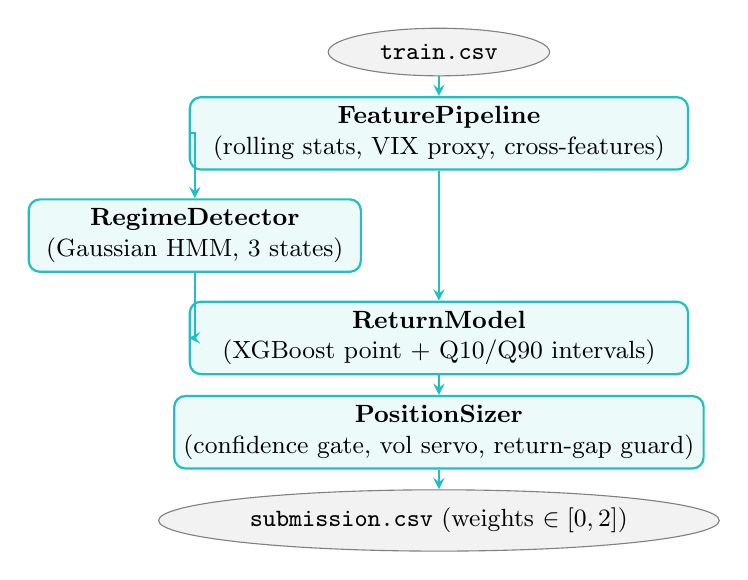
\begin{tikzpicture}[
    node distance=0.25cm and 0.5cm,
    block/.style={draw=kaggleteal, fill=kaggleteal!8, rectangle, rounded corners, minimum height=1.4em, minimum width=18em, align=center, thick, font=\small},
    smallblock/.style={draw=kaggleteal, fill=kaggleteal!8, rectangle, rounded corners, minimum height=1.4em, minimum width=12em, align=center, thick, font=\small},
    io/.style={draw=gray, fill=gray!10, ellipse, minimum height=1.2em, minimum width=8em, align=center, font=\small},
    arrow/.style={thick, ->, >=stealth, draw=kaggleteal}
]
    % Nodes
    \node (input) [io] {\texttt{train.csv}};
    \node (pipeline) [block, below=0.25cm of input] {\textbf{FeaturePipeline} \\ (rolling stats, VIX proxy, cross-features)};
    \node (regime) [smallblock, below left=0.35cm and -2.2cm of pipeline] {\textbf{RegimeDetector} \\ (Gaussian HMM, 3 states)};
    \node (model) [block, below=1.65cm of pipeline] {\textbf{ReturnModel} \\ (XGBoost point + Q10/Q90 intervals)};
    \node (sizer) [block, below=0.25cm of model] {\textbf{PositionSizer} \\ (confidence gate, vol servo, return-gap guard)};
    \node (output) [io, below=0.25cm of sizer] {\texttt{submission.csv} (weights $\in [0, 2]$)};

    % Arrows
    \draw [arrow] (input) -- (pipeline);
    \draw [arrow] (pipeline.west) -| (regime.north);
    \draw [arrow] (pipeline.south) -- (model.north);
    \draw [arrow] (regime.south) |- (model.west);
    \draw [arrow] (model) -- (sizer);
    \draw [arrow] (sizer) -- (output);
\end{tikzpicture}
\end{center}
\end{frame}

% ===== Slide 7: Feature Engineering =====
\begin{frame}{Feature Engineering}
\small
\begin{columns}[T]
\begin{column}{0.48\textwidth}
\textbf{Rolling Statistics}
\begin{itemize}
    \item Volatility: $\sigma_{5,20,60,252}$
    \item Momentum: $r_{5,20,60,252}$
    \item Sharpe ratios: $\text{SR}_{20,60}$
    \item Drawdown: $\text{DD}_{60}$, $\text{MaxDD}_{252}$
\end{itemize}
\vspace{0.2cm}
\textbf{VIX Features}
\begin{itemize}
    \item VIX Proxy: mean of V1--V13
    \item Percentile rank (train-frozen)
    \item Term-slope: V13 $-$ V1
    \item VIX delta (history-buffered)
\end{itemize}
\end{column}
\begin{column}{0.48\textwidth}
\textbf{Cross-Features}
\begin{itemize}
    \item Yield-curve proxy: $I_{\text{last}} - I_{\text{first}}$
    \item Macro-sentiment divergence
    \item Price-momentum agreement
    \item Autocorrelation: $\rho_{5,20}$
\end{itemize}
\vspace{0.2cm}
\textbf{Anti-Leakage}
\begin{itemize}
    \item Median imputation: train medians only
    \item 400-row history buffer for rolling windows
    \item Lagged targets only: \texttt{.shift(1)}
\end{itemize}
\end{column}
\end{columns}
\vspace{0.3cm}
\textbf{Total}: $\sim$107 engineered features after availability filtering.
\end{frame}

% ===== Slide 8: Volatility Proxy =====
\begin{frame}{Volatility Proxy}
\begin{itemize}
    \item The V1--V13 columns in \texttt{train.csv} are anonymized volatility features
    \item A simple proxy maps V1--V13 into a unified volatility level
    \item Calculated as the cross-sectional mean: $\text{VIX Proxy}_t = \frac{1}{13} \sum_{i=1}^{13} V_{i, t}$
\end{itemize}
\vspace{0.15cm}
\begin{block}{Why a proxy?}
    VIX is a well-known fear gauge. Compressing the volatility dimensions recovers a signal that is:
    \begin{itemize}
        \item Statistically associated with future volatility
        \item A useful volatility signal for this dataset
        \item Useful for regime detection and risk-aware position sizing
    \end{itemize}
\end{block}
\vspace{0.15cm}
Four features are derived from the VIX proxy:
\begin{enumerate}
    \item \textbf{VIX proxy}, cross-sectional mean level signal
    \item \textbf{VIX percentile rank}, where current VIX sits vs.\ historical distribution
    \item \textbf{VIX term-slope}, V13 $-$ V1 (volatility term structure)
    \item \textbf{VIX delta}, day-over-day change (momentum of fear)
\end{enumerate}
\end{frame}


% ==============================================================================
% SECTION 3: Market Regime Detection
% ==============================================================================
\section{Market Regime Detection}

% ===== Slide 9: Regime Detection =====
\begin{frame}{Market Regime Detection}
\begin{itemize}
    \item \textbf{Gaussian HMM} with 3 hidden states, diagonal covariance
    \item Inputs: \texttt{vix\_proxy\_pct}, \texttt{roll\_vol\_20}, \texttt{momentum\_20}, \texttt{autocorr\_20}

\end{itemize}
\vspace{0.2cm}
\begin{block}{Output per row}
    \begin{itemize}
        \item \texttt{regime\_state}, Viterbi-decoded hidden state
        \item \texttt{regime\_prob\_\{0,1,2\}}, posterior probabilities
        \item \texttt{regime\_stability}, confidence in regime assignment
        \item \texttt{regime\_label}, semantic labels (e.g. \texttt{bull\_low\_vol}, \texttt{bear\_high\_vol}) assigned by training set mean return/volatility comparisons
    \end{itemize}
\end{block}
\end{frame}


% ==============================================================================
% SECTION 4: Model \& Trading Strategy
% ==============================================================================
\section{Model \& Trading Strategy}

% ===== Slide 10: Return Prediction Model =====
\begin{frame}{Return Prediction Model (XGBoost)}
Three models trained simultaneously on \texttt{market\_forward\_excess\_returns}:
\vspace{0.15cm}
\begin{center}
\small
\begin{tabular}{lcc}
\toprule
\textbf{Model} & \textbf{Objective} & \textbf{Purpose} \\
\midrule
Point model   & \texttt{reg:squarederror}  & Direction \& magnitude \\
Lower quantile (Q10) & \texttt{reg:quantileerror}, $\alpha=0.1$ & Lower bound \\
Upper quantile (Q90) & \texttt{reg:quantileerror}, $\alpha=0.9$ & Upper bound \\
\bottomrule
\end{tabular}
\end{center}
\vspace{0.2cm}
\textbf{Confidence signal}:
\[
\text{raw\_conf} = \frac{|\text{point\_pred}|}{\max(\text{Q90} - \text{Q10},\; \varepsilon)} \quad \longrightarrow \quad
\text{confidence} = \operatorname{clip}\!\left(\frac{\text{raw\_conf} - p_{10}}{p_{90} - p_{10}},\; 0,\; 1\right)
\]
\vspace{0.1cm}
Percentiles $p_{10}, p_{90}$ are computed on training data and frozen. This maps raw confidence to $[0,1]$, filtering noise while preserving relative ordering.
\end{frame}

% ===== Slide 11: Model Hyperparameters =====
\begin{frame}{Model Hyperparameters \& Regularization}
\begin{columns}[T]
\begin{column}{0.48\textwidth}
\textbf{XGBoost parameters}
\begin{itemize}
    \item \texttt{max\_depth = 4}
    \item \texttt{learning\_rate = 0.05}
    \item \texttt{subsample = 0.8}
    \item \texttt{colsample\_bytree = 0.8}
\end{itemize}
\end{column}
\begin{column}{0.48\textwidth}
\textbf{Tree Count \& Regularization}
\begin{itemize}
    \item Point model uses \textbf{400 trees} to learn directional signal
    \item Quantile bounds are limited to \textbf{150 trees} ($\frac{1}{3}$ of point)
    \item Shorter ensembles act as early stopping to prevent overfitting to noisy tails
\end{itemize}
\end{column}
\end{columns}
\vspace{0.3cm}
\textbf{Purged Walk-Forward CV}: Time-series cross-validation with a configurable purge gap between each training window and validation fold, preventing any forward information leakage through autocorrelated targets.
\end{frame}

% ===== Slide 12: Position Sizing =====
\begin{frame}{Confidence-Gated Position Sizing}
\begin{columns}[T]
\begin{column}{0.62\textwidth}
\textbf{Two-branch logic per time step}:
\[
\begin{cases}
w = 1.0, & \text{if confidence} < \text{threshold}\\[3pt]
w = 1.0 + \text{gain} \times \text{pred} \times \text{vol\_scale} \times \text{reg\_mult}, & \text{otherwise}
\end{cases}
\]
\vspace{0.1cm}
\textbf{Volatility scaling} (Moreira \& Muir, 2017):
\[
\text{vol\_scale} = \operatorname{clip}\!\left(\frac{\sigma_{\text{target}}}{\sigma_t},\; 0.5,\; 2.0\right)
\]
\end{column}
\begin{column}{0.36\textwidth}
\textbf{Regime multipliers}
\vspace{0.15cm}
\begin{center}
\small
\begin{tabular}{lr}
\toprule
\textbf{Regime} & \textbf{Multiplier} \\
\midrule
Bull, low volatility   & 1.30 \\
Normal                 & 1.00 \\
Transition             & 0.70 \\
Bear, high volatility  & 0.50 \\
\bottomrule
\end{tabular}
\end{center}
\end{column}
\end{columns}
\vspace{0.25cm}
\begin{block}{Rationale}
    The strategy stays at baseline exposure when confidence is low, scales risk inversely to volatility, and reduces active bets in unstable or high-volatility regimes.
\end{block}
\end{frame}

% ===== Slide 13: Runtime Guards =====
\begin{frame}{Runtime Guards}
Two sequential guards applied after the base weight calculation:

\begin{itemize}
    \item \textbf{Volatility servo}: If rolling strategy vol / market vol exceeds 1.149 (soft cap) or 1.20 (hard cap), active deviation is scaled back to 55\% or 20\% to avoid the vol penalty.
    \item \textbf{Return-gap guard}: If strategy return falls behind the market, force $w \geq 1.0$ to prevent further divergence and avoid the quadratic return penalty.
\end{itemize}

\vspace{0.2cm}
\begin{block}{Defensive Mechanism}
    The quadratic return penalty makes underperformance costly. Guards act defensively, reducing downside risk without removing the strategy's upside exposure.
\end{block}
\end{frame}


% ==============================================================================
% SECTION 5: Validation \& Results
% ==============================================================================
\section{Validation \& Results}

% ===== Slide 14: Walk-Forward Validation =====
\begin{frame}{Walk-Forward Backtesting}
\begin{itemize}
    \item Each CV fold re-fits the \textbf{entire modeling pipeline} independently
    \item Features, regime detector, and return model are all refit from scratch per fold
    \item No state, scaler, or model weight is shared between folds
    \item Model predictions are cached; strategy parameters are then scored with the exact competition metric
\end{itemize}
\vspace{0.15cm}
\begin{block}{Fold-by-Fold Validation Diagnostics}
    \begin{center}
    \scriptsize
    \begin{tabular}{ccccc}
        \toprule
        \textbf{Fold} & \textbf{Validation Range} & \textbf{Adj.\ Sharpe} & \textbf{Mean Weight} & \textbf{Dominant Regime} \\
        \midrule
        1 & 3\,790 -- 4\,372 & +0.9985 & 0.914 & Transition \\
        2 & 4\,373 -- 4\,955 & -0.2741 & 1.136 & Transition \\
        3 & 4\,956 -- 5\,538 & +0.8578 & 0.981 & Bear (High Vol) \\
        4 & 5\,539 -- 6\,121 & +1.5707 & 1.012 & Transition \\
        5 & 6\,122 -- 6\,704 & +0.9661 & 0.950 & Bear (High Vol) \\
        6 & 6\,705 -- 7\,287 & +0.9965 & 0.930 & Transition \\
        \bottomrule
    \end{tabular}
    \end{center}
\end{block}
\end{frame}

% ===== Slide 15: Hyperparameter Tuning =====
\begin{frame}{Strategy Tuning}
\begin{itemize}
    \item The model pipeline is fixed before tuning strategy parameters
    \item Inner CV fold predictions are cached once to avoid refitting the model for every trial
    \item Optuna runs \textbf{40 strategy-only trials} over confidence threshold, gain, target volatility, and soft volatility cap
    \item Initial untuned strategy mean CV adjusted Sharpe: \textbf{0.7246}
    \item Best inner CV mean adjusted Sharpe: \textbf{0.8526}
\end{itemize}
\vspace{0.2cm}
\begin{block}{Why cache folds?}
    The expensive feature, regime, and return-model steps are fitted once per fold. Optuna then evaluates only the lightweight weight-generation rule, so the search remains reproducible and fast.
\end{block}
\end{frame}

% ===== Slide 16: Results =====
\begin{frame}{Holdout Results}
\begin{center}
\small
\begin{tabular}{lcccc}
\toprule
\textbf{Configuration} & \textbf{Adj.\ Sharpe} & \textbf{Ann.\ Return} & \textbf{Vol Ratio} & \textbf{Active Days} \\
\midrule
This model (Tuned) & \textbf{0.8605} & \textbf{+20.2\%} & 1.020 & 29.5\% \\
Baseline ($w=1.0$) & 0.7151          & +16.8\%          & 1.000 & --    \\
\midrule
\textbf{Delta}     & \textbf{+0.1454} & \textbf{+3.4 pp} &       &        \\
\bottomrule
\end{tabular}
\end{center}
\vspace{0.3cm}
\begin{itemize}
    \item \textbf{+20.3\%} improvement in adjusted Sharpe over baseline on untouched holdout
    \item Inner CV mean adjusted Sharpe: \textbf{0.8526} (6 folds)
    \item Only 29.5\% of days are active, so most days stay close to baseline exposure
    \item Tuned parameters: confidence threshold = 0.364, gain = 179.3, target vol = 0.298, soft vol cap = 1.149
\end{itemize}
\end{frame}

% ===== Slide 17: Leakage Prevention =====
\begin{frame}{Leakage Prevention}
\begin{table}
\footnotesize
\begin{tabular}{p{4.8cm}p{7.2cm}}
\toprule
\textbf{Risk} & \textbf{Mitigation} \\
\midrule
Feature leakage from future & \texttt{fit\_transform} on training only; apply frozen stats \\
Rolling boundary leakage & 400-row history buffer prepended to validation/holdout blocks \\
Temporal lookahead in CV & Purged walk-forward CV; separate 200-day purge before final holdout \\
Target leakage & Lagged targets only (\texttt{.shift(1)}); target excluded from features \\
Tuning lookahead & Hyperparameters tuned on inner temporal holdout \\
XGBoost non-determinism & Enforce \texttt{nthread=1}, \texttt{tree\_method='hist'}, \texttt{seed=42} \\
\bottomrule
\end{tabular}
\end{table}
\vspace{0.15cm}
\begin{block}{Critical Importance}
    Strict anti-leakage controls prevent inflated backtest performance. Purge gaps and history buffering are mandatory for reliable time-series modeling.
\end{block}
\end{frame}

% ===== Slide 18: Reproducibility =====
\begin{frame}{Reproducibility \& Design Notes}
\textbf{Reproducibility measures}:
\begin{itemize}
    \item All random seeds: \texttt{42} (XGBoost, sklearn, HMM)
    \item XGBoost: \texttt{nthread=1}, \texttt{tree\_method='hist'} for cross-platform determinism
    \item Log \texttt{holdout\_size} and \texttt{purge\_gap} with every experiment
\end{itemize}
\vspace{0.3cm}
\textbf{Why only 29.5\% active days?}
\begin{itemize}
    \item The confidence threshold is high, as most days the prediction interval is wide relative to the point estimate
    \item Active days cluster around high-confidence signals: trend-consistent predictions during low-volatility bull regimes
    \item Index-tracking as the default absorbs return-gap risk; the strategy can only improve the score by being active
\end{itemize}
\end{frame}

% ===== Slide 19: Summary =====
\begin{frame}{Summary}
\textbf{Key Takeaways}:
\begin{itemize}
    \item The adjusted Sharpe's quadratic return penalty fundamentally shapes the strategy design.
    \item Confidence-gating is essential: default to the index unless high confidence is present.
    \item Volatility management (Moreira \& Muir, 2017) boosts Sharpe ratio by scaling risk dynamically.
    \item HMM-based regime detection provides context to optimize position sizing.
    \item Purged walk-forward validation is mandatory to estimate real out-of-sample performance.
\end{itemize}
\end{frame}

% ===== Slide 20: References =====
\begin{frame}{References}
\textbf{References}:
\begin{itemize}
    \item Moreira, A. \& Muir, T. (2017). \textit{Volatility-Managed Portfolios}. Journal of Finance, 72(4), 1611--1644.
    \item Kaggle Competition: \url{https://www.kaggle.com/competitions/hull-tactical-market-prediction}
    \item Chen, T. \& Guestrin, C. (2016). \textit{XGBoost: A Scalable Tree Boosting System}. KDD 2016.
\end{itemize}
\end{frame}

\end{document}
